% Unofficial UChicago CS Poster Template
% v1.1.0 released September 8, 2022
% https://github.com/k4rtik/uchicago-poster
% a fork of https://github.com/anishathalye/gemini

\documentclass[final]{beamer}

% ====================
% Packages
% ====================

\usepackage[T1]{fontenc}
\usepackage{lmodern}
\usepackage[size=A0,orientation=portrait,scale=1.00]{beamerposter}
\usetheme{gemini}
\usecolortheme{uchicago}
\usepackage{graphicx}
\usepackage{epstopdf}
\usepackage{booktabs}
\usepackage{doi}
\usepackage[numbers]{natbib}
\usepackage[patch=none]{microtype}
\usepackage{tikz}
\usepackage{quantikz}
\usepackage{pgfplots}
\pgfplotsset{compat=1.18}
\usepackage{anyfontsize}
\usepackage{physics}
\usepackage{subcaption}

% TikZ libraries
\usetikzlibrary{decorations.pathreplacing}

\pdfstringdefDisableCommands{%
\def\translate#1{#1}%
\def\inst#1{}%
}

% ====================
% Lengths
% ====================

% If you have N columns, choose \sepwidth and \colwidth such that
% (N+1)*\sepwidth + N*\colwidth = \paperwidth
\newlength{\sepwidth}
\newlength{\colwidth}
\setlength{\sepwidth}{0.04\paperwidth}
\setlength{\colwidth}{0.44\paperwidth}

\newcommand{\separatorcolumn}{\begin{column}{\sepwidth}\end{column}}

% ====================
% Title
% ====================

\title{Enhanced Electron Nuclear Spin Control Leveraging Hyperfine Coupling and Radio-Frequency Drive}

\author{Donghun Jung\inst{1, }\inst{2}, Eunsang Lee\inst{1}, Jiwon Jeon\inst{1}, Junghyun Lee\inst{1, $\dagger$}}

\institute[shortinst]{\inst{1} Center for Quantum Information, Korea Institute of Science and Technology, Seoul 02792, Republic of Korea \linebreak \inst{2} Department of Physics, Sungkyunkwan University, Suwon 16419, Republic of Korea}

% ====================
% Footer (optional)
% ====================

\footercontent{
  \href{https://sites.google.com/view/pauleegroup}{https://sites.google.com/view/pauleegroup} \hfill
  Quantum Information Society of Korea \hfill
  \href{mailto:jh_lee@kist.re.kr}{$\dagger$ jh\_lee@kist.re.kr}}
  % (can be left out to remove footer)

% ====================
% Logo (optional)
% ====================

% use this to include logos on the left and/or right side of the header:
% \logoright{\includegraphics[height=7cm]{logo1.pdf}}
% \logoleft{\includegraphics[height=7cm]{logo2.pdf}}

% ====================
% Body
% ====================

\logoleft{
\includegraphics[height=4.0cm]{logos/KIST_CI.eps}}
\logoright{
\includegraphics[height=2.5cm]{logos/PaulLee2.eps}}

\begin{document}

\begin{frame}[t]
\begin{columns}[t]
\separatorcolumn

\begin{column}{\colwidth}
  \begin{alertblock}{Abstract}

  Solid-state defect systems have emerged as promising platforms for quantum information processing and sensing.
  In particular, the nitrogen-vacancy (NV) center in diamond, coupled with surrounding nuclear spins, exhibits long coherence times and enables high-fidelity operations.
  To implement high-fidelity, selective-qubit operations, dynamic decoupling (DD) sequences, consisting of multi-pulse control on the NV spin, have been developed to achieve entangling gates with selected target nuclear spins while reducing decoherence from the broader spin bath.
  On the other hand, an additional selective phase-controlled radio-frequency (rf) driving on nuclear spins, referred as DDrf gate, enables elaborated control of individual spins.
  The mechanisms underlying these approaches differ that dynamic decoupling relies on transverse hyperfine interaction components, whereas the DDrf gate exploits rf driving and suppresses transverse hyperfine coupling.
  In this work, we propose a hybrid DDrf gate that leverages both mechanisms to achieve faster and more robust gate operations.
  The hybrid gate achieves faster and more robust operations than either the DD or DDrf approach alone, and extends high-fidelity control to nuclear spins with weak transverse hyperfine coupling.

  \end{alertblock}


  \begin{block}{Nitrogen-Vacancy (NV) center system}
  In the nitrogen-vacancy (NV) center, such an operation can be implemented by a sort of Hamiltonian engineering.
  We consider a nitrogen-vacancy (NV) center electron spin ($S = 1$) coupled to surrounding $^{13}$C nuclear spins $(I=\frac{1}{2})$ via the hyperfine interaction~\cite{taminiau2012}.
  The Hamiltonian is
  $$
  H = \ketbra{0} \otimes \underbrace{\omega_0 I_z}_{= H_0}+ \ketbra{1} \otimes \underbrace{ (\omega_0 - A_\parallel)\, I_z + A_\perp\, I_x}_{= H_1}
  $$
  where $\omega_0$ is the nuclear Larmor frequency, and $A_\parallel$, $A_\perp$ are the parallel and perpendicular hyperfine components.
  We can evaluate the time evolution of the $^{13}$C nuclear spin depending on the NV center electron spin state in a piecewise manner.
  \end{block}


  % \begin{block}{Conditional Gate}
  % % Beyond a mere collection of independent qubits, entanglement between the qubits is regarded as a core resource for quantum computing.
  % % Two-qubit gates are the source of entanglement between qubits, so implementing two-qubit gates in a particular physical quantum system is of critical interest.
  % % Generally such an operation can be implemented by conditional operation, that is, a two-qubit gate acts on a control qubit and a target qubit.
  % The operation applied to the target depends on the state of the control qubit, and can be written as:
  % $$
  % U = \ketbra{0} \otimes U_0 + \ketbra{1} \otimes U_1,
  % $$
  % where $U_0$ and $U_1$ are single-qubit rotations conditioned on the control qubit state.
  % % Without loss of generality, we can write each operation as $e^{-i \theta_{i} \vec{\sigma}_{i}}$.
  % % When the rotating axes $\vec{\sigma}$ on the target qubit are significantly different, or even antiparallel, the gate operation becomes conditional, ultimately generating entanglement.
  % \end{block}

  \begin{block}{Dynamic Decoupling (DD)}
    We can enable conditional interaction by applying a dynamic decoupling sequence consisting of $N$ sequential $\pi$-pulses.
    Consider the basic decoupling unit on the electron spin $\tau$-$\pi$-$2\tau$-$\pi$-$\tau$ where $\tau$ is a free evolution time.

    \heading{CPMG Pulse Sequence}

    \begin{figure}
      \centering
      \begin{minipage}[c]{0.57\linewidth}
        \centering
        \begin{tikzpicture}[xscale=3.5, yscale=2.0]
          % Baseline
          \draw[thick] (0, 0) -- (3.8, 0);
          \node[left, font=\small\bfseries] at (-0.05, 0.45) {MW};
          % Dots
          \node[font=\Large] at (0.25, 0.40) {$\cdots$};
          % π/2 pulse
          % \fill[blue!60] (0.20, 0) rectangle (0.38, 0.8);
          % \node[above, font=\small] at (0.29, 0.85) {$\frac{\pi}{2}$};
          % τ
          \draw[<->, thin] (0.42, -0.18) -- (0.95, -0.18);
          \node[below, font=\small] at (0.685, -0.22) {$\tau$};
          % First π pulse
          \fill[purple!70] (1.00, 0) rectangle (1.18, 0.8);
          \node[above, font=\small] at (1.09, 0.85) {$\pi$};
          % 2τ
          \draw[<->, thin] (1.22, -0.18) -- (2.10, -0.18);
          \node[below, font=\small] at (1.66, -0.22) {$2\tau$};
          % Second π pulse
          \fill[purple!70] (2.15, 0) rectangle (2.33, 0.8);
          \node[above, font=\small] at (2.24, 0.85) {$\pi$};
          % τ
          \draw[<->, thin] (2.37, -0.18) -- (2.90, -0.18);
          \node[below, font=\small] at (2.635, -0.22) {$\tau$};
          % Brace for unit
          \draw[decorate, decoration={brace, amplitude=6pt, mirror}]
            (0.42, -0.65) -- (2.90, -0.65)
            node[midway, below=8pt, font=\small] {$(\tau\text{-}\pi\text{-}2\tau\text{-}\pi\text{-}\tau)^{N/2}$};
          % Dots
          \node[font=\Large] at (3.45, 0.40) {$\cdots$};
          % -π/2 pulse
          % \fill[blue!60] (3.95, 0) rectangle (4.13, 0.8);
          % \node[above, font=\small] at (4.04, 0.85) {$-\frac{\pi}{2}$};
        \end{tikzpicture}
      \end{minipage}%
      \hfill
      \begin{minipage}[c]{0.40\linewidth}
        \centering
        \begin{quantikz}[row sep=1.3cm, column sep=0.7cm]
          \lstick{$\mathrm{NV}^{-}$} & \ctrl{1} & \ctrl{1} & \qw \rstick{$\cdots$} \\
          \lstick{${}^{13}\mathrm{C}$} & \gate{U(\tau)} & \gate{U(\tau)} & \qw \rstick{$\cdots$}
        \end{quantikz}
      \end{minipage}
      \caption{CPMG dynamical decoupling sequence on the NV electron spin (left) and equivalent quantum circuit (right).}
    \end{figure}

    The net result of this unit sequence results in a rotation by an angle $\phi$ around an axis $\vec{\sigma}_{i}$, depending on the initial state of the electron spin;
    $\vec{\sigma}_0$ for $m_s = 0$ state, and
    $\vec{\sigma}_1$ for $m_s = -1$ state.
    If $\vec{\sigma}_0$ and $\vec{\sigma}_1$ are not parallel, the resulting conditional rotation of the nuclear spin generally entangles the electron and nuclear spins.
    A dynamical decoupling sequence with the basic unit $\tau$-$\pi$-$2\tau$-$\pi$-$\tau$, repeated $N/2$ times, makes further conditional operation.

    \heading{Conditional Rotation \& Resonance}

    \begin{figure}[c]
      \centering
      \begin{subfigure}[c]{0.5\linewidth}
        \centering
        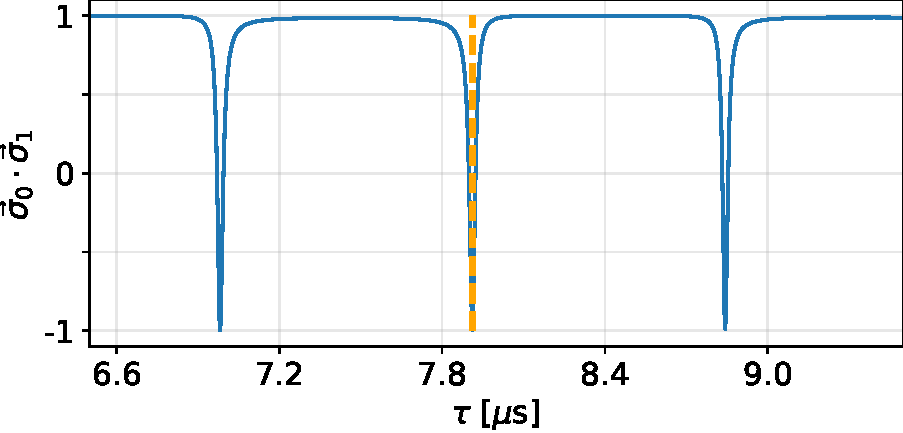
\includegraphics[width=\linewidth]{media/fig1.pdf}
      \end{subfigure}
      \begin{subfigure}[c]{0.3\linewidth}
        \centering
        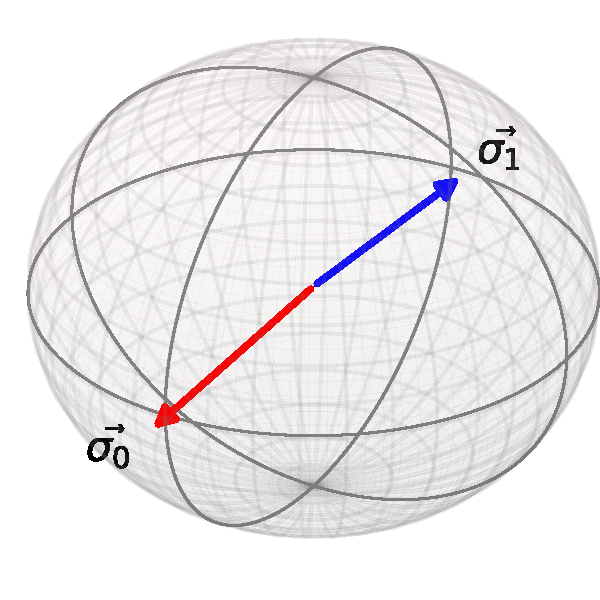
\includegraphics[width=\linewidth]{media/fig2.pdf}
      \end{subfigure}
      \caption{(Left) Inner product $\vec{\sigma}_0 \cdot \vec{\sigma}_1$ as a function of $\tau$, showing sharp resonances where the axes become antiparallel; the orange dashed line marks the chosen $\tau_k$. (Right) Conditional rotation axes $\vec{\sigma}_0$ (red) and $\vec{\sigma}_1$ (blue) on the Bloch sphere at resonance.}
    \end{figure}

    The conditional evolution operators for a single decoupling unit are:
    \begin{align}
      U_0 &= e^{-i\tau H_0}e^{-i2\tau H_1}e^{-i\tau H_0} = e^{-i\phi_{\text{DD}} \vec{\sigma}_0} \\
      U_1 &= e^{-i\tau H_1}e^{-i2\tau H_0}e^{-i\tau H_1} = e^{-i\phi_{\text{DD}} \vec{\sigma}_1}
    \end{align}
    Here $\omega_0 \equiv \omega_0$ and $\omega_1 = \sqrt{(\omega_0 + A_\parallel)^2 + A_\perp^2}$ are the nuclear precession frequencies for $m_s = 0$ and $m_s = -1$, respectively.
    The conditional rotation angle $\phi_{\text{DD}}$ and inner product between the two rotation axes are determined by the choice of $\tau$ and NV center system configuration.
    \begin{align}
      \cos\phi_{\text{DD}} &= \cos \omega_1 \tau \cos\omega_0 \tau - \frac{\omega_0 - A_{\parallel}}{\omega_1} \sin \omega_1 \tau \sin\omega_0 \tau \\
      1 - \vec{\sigma}_0 \cdot \vec{\sigma}_1 &= \frac{A_{\perp}^2}{\omega_0^2} \frac{(1-\cos\omega_1 \tau)(1-\cos\omega_0 \tau)}{1 + \cos\phi_{\text{DD}}}
    \end{align}
    % This simple implementation has limit (discretization, passive operation(contingent onf A_perp))

    % \heading{Spectroscopy}

    \begin{figure}
      \centering
      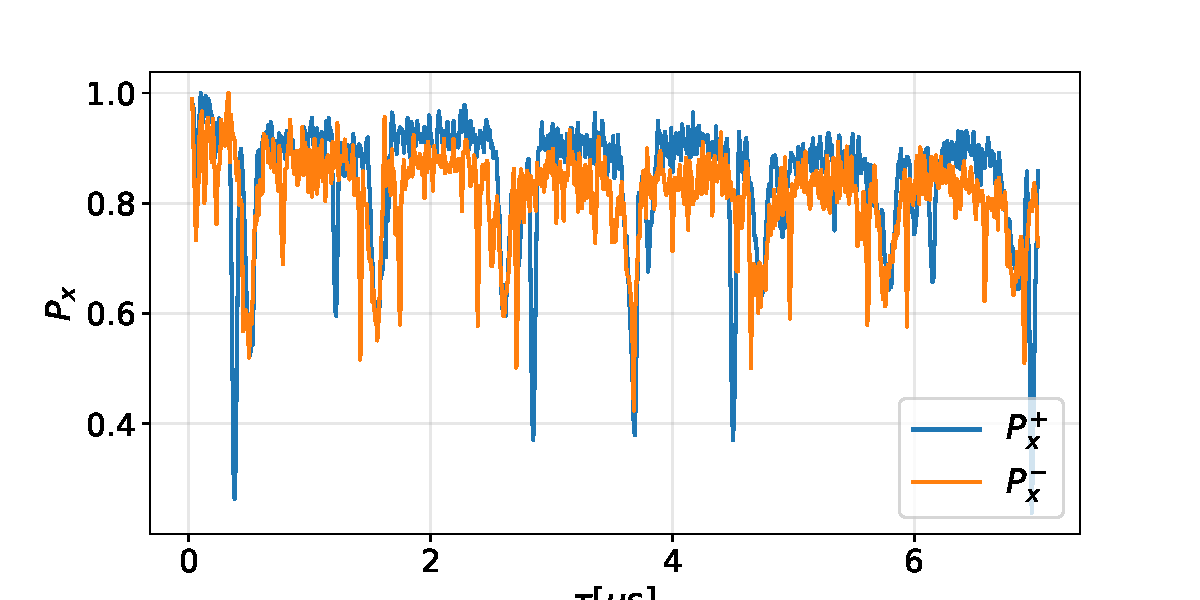
\includegraphics[width=0.7\linewidth]{media/CPMG.pdf}
      \caption{
        $\ket{+}$-state projection ($P_x$) of the CPMG sequence, with the NV electron spin initialized to $\ket{+}$ and the $^{13}$C nuclear spins in a fully mixed state.
        The sharp resonances in the echo signal arise from coherent interaction with individual $^{13}$C nuclear spins.
      }
    \end{figure}

  \end{block}
\end{column}

\separatorcolumn

\begin{column}{\colwidth}

  \begin{block}{DDrf Gate}

    The DDrf gate combines dynamical decoupling on the electron spin with phase-controlled radio-frequency (rf) driving of the nuclear spin~\cite{bradley2019}.

    \heading{Hamiltonian}
    In the interaction picture and rotating frame with respect to the electron energy splitting and neglecting non-secular terms, the Hamiltonian of the NV-$^{13}C$ system under the approximation $A_\perp \approx 0$ and $\Omega_{\text{RF}} \ll (\omega_0 - \omega_1)$ is given
    \begin{align}
      H = \ketbra{0} \otimes \underbrace{(\omega_0 - \omega_1 )I_z}_{=H_0} + \ketbra{1} \otimes \underbrace{\Omega_{\text{RF}}( \cos\phi I_x + \sin\phi I_y )}_{=H_1}.
    \end{align}
    where the final term describes the interaction of the nuclear spin with a radio frequency (RF) driving field polarized along the $x$ axis (in the same direction as the hyperfine coupling), phase $\phi$ and Rabi frequency $\Omega_{\text{RF}}$.

    \heading{Pulse Sequence}
    \begin{figure}
      \centering
      \begin{minipage}[c]{0.55\linewidth}
        \centering
        \begin{tikzpicture}[xscale=2.8, yscale=1.8]
          % Labels
          \node[left, font=\small\bfseries] at (-0.15, 1.65) {MW};
          \node[left, font=\small\bfseries] at (-0.15, 0.30) {rf};
          % MW line
          \draw[thick] (0, 1.3) -- (6.3, 1.3);
          % rf line
          \draw[thick] (0, 0) -- (6.3, 0);
          %
          % Layout: rf pulses fill the full gaps between pi-pulses.
          % One unit = rf1(tau) - pi1 - rf2(2tau) - pi2 - half of rf3(tau).
          % The underbrace spans from start of rf1 to middle of rf3.
          %
          % rf_1 (odd, red) — width tau
          \fill[red!40] (0.00, 0) rectangle (0.55, 0.55);
          \node[below, font=\scriptsize] at (0.275, -0.05) {$1$};
          \node[below, font=\scriptsize] at (0.275, 0.55) {$\phi_1$};
          % pi_1
          \fill[purple!70] (0.55, 1.3) rectangle (0.72, 2.0);
          \node[above, font=\small] at (0.635, 2.05) {$\pi$};
          % rf_2 (even, blue) — width 2tau
          \fill[blue!40] (0.72, 0) rectangle (1.82, 0.55);
          \node[below, font=\scriptsize] at (1.27, -0.05) {$2$};
          \node[below, font=\scriptsize] at (1.27, 0.55) {$\phi_2$};
          % pi_2
          \fill[purple!70] (1.82, 1.3) rectangle (1.99, 2.0);
          \node[above, font=\small] at (1.905, 2.05) {$\pi$};
          % rf_3 (odd, red) — width 2tau, straddles unit boundary at midpoint 2.54
          \fill[red!40] (1.99, 0) rectangle (3.09, 0.55);
          \node[below, font=\scriptsize] at (2.54, -0.05) {$3$};
          \node[below, font=\scriptsize] at (2.54, 0.55) {$\phi_3$};
          % pi_3
          \fill[purple!70] (3.09, 1.3) rectangle (3.26, 2.0);
          \node[above, font=\small] at (3.175, 2.05) {$\pi$};
          % rf_4 (even, blue) — width 2tau
          \fill[blue!40] (3.26, 0) rectangle (4.36, 0.55);
          \node[below, font=\scriptsize] at (3.81, -0.05) {$4$};
          \node[below, font=\scriptsize] at (3.81, 0.55) {$\phi_3$};
          % Dots
          \node[font=\Large] at (5.05, 0.3) {$\cdots$};
          % rf_K (odd, red) — width tau
          \fill[red!40] (5.75, 0) rectangle (6.30, 0.55);
          \node[below, font=\scriptsize] at (6.025, -0.05) {$K$};
          \node[below, font=\scriptsize] at (6.025, 0.55) {$\phi_K$};
          % tau and 2tau arrows (between MW and rf lines)
          \draw[<->, thin] (0.00, 0.80) -- (0.55, 0.80);
          \node[above, font=\scriptsize] at (0.275, 0.83) {$\tau$};
          \draw[<->, thin] (0.72, 0.80) -- (1.82, 0.80);
          \node[above, font=\scriptsize] at (1.27, 0.83) {$2\tau$};
          \draw[<->, thin] (1.99, 0.80) -- (3.09, 0.80);
          \node[above, font=\scriptsize] at (2.54, 0.83) {$2\tau$};
          % Underbrace: start of rf1 to middle of rf3 (one unit = 2 pi-pulses)
          \draw[decorate, decoration={brace, amplitude=6pt, mirror}]
            (0.00, -0.45) -- (2.54, -0.45)
            node[midway, below=8pt, font=\small] {$(\tau\text{-}\pi\text{-}2\tau\text{-}\pi\text{-}\tau)^{N/2}$};
          % Legend — stacked on the left to avoid overflow
          \fill[red!40] (0.0, -1.55) rectangle (0.30, -1.30);
          \node[right, font=\scriptsize] at (0.35, -1.425) {odd $k$: resonant for $\ket{1}$ ($m_s = -1$)};
          \fill[blue!40] (0.0, -1.95) rectangle (0.30, -1.70);
          \node[right, font=\scriptsize] at (0.35, -1.825) {even $k$: resonant for $\ket{0}$ ($m_s = 0$)};
        \end{tikzpicture}
      \end{minipage}%
      \hfill
      \begin{minipage}[c]{0.42\linewidth}
        \centering
        \begin{quantikz}[row sep=1.1cm, column sep=0.4cm]
          \lstick{$\mathrm{NV}^{-}$} & \qw & \ctrl{1} & \qw & \ctrl{1} & \qw \rstick{$\cdots$} \\
          \lstick{${}^{13}\mathrm{C}$} & \gate{R_z} & \gate{\substack{R_{\varphi} \\ (\pm\Omega\tau)}} & \gate{R_z} & \gate{\substack{R_{\varphi} \\ (\pm\Omega\tau)}} & \qw \rstick{$\cdots$}
        \end{quantikz}
      \end{minipage}
      \caption{DDrf pulse sequence: MW $\pi$-pulses interleaved with phase-controlled rf pulses (left); equivalent quantum circuit showing the conditional $R_\varphi(\pm\Omega\tau)$ rotation per unit (right).}
    \end{figure}

    The electron spin state determines which rf pulses are resonant: odd-$k$ pulses drive the nuclear spin when the electron is in $\ket{1}$ ($m_s = -1$), while even-$k$ pulses are resonant for $\ket{0}$ ($m_s = 0$).
    The rf pulse phases $\phi_k = \varphi + \phi_k'$ are set to accumulate constructive rotations:
    $$
    \phi_k' = \begin{cases} (k-1)\phi_\tau + \pi, & k \text{ odd} \\ (k-1)\phi_\tau, & k \text{ even} \end{cases}, \qquad \phi_\tau = A_\parallel \tau.
    $$

    \heading{Controlled Rotation}
    \begin{figure}[c]
      \centering
      \begin{subfigure}[c]{0.3\linewidth}
        \centering
        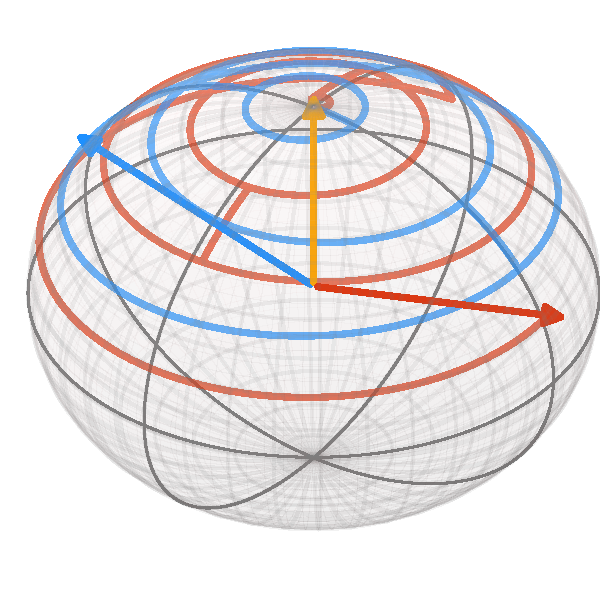
\includegraphics[width=\linewidth]{media/DDrf_1.pdf}
      \end{subfigure}
      \begin{subfigure}[c]{0.3\linewidth}
        \centering
        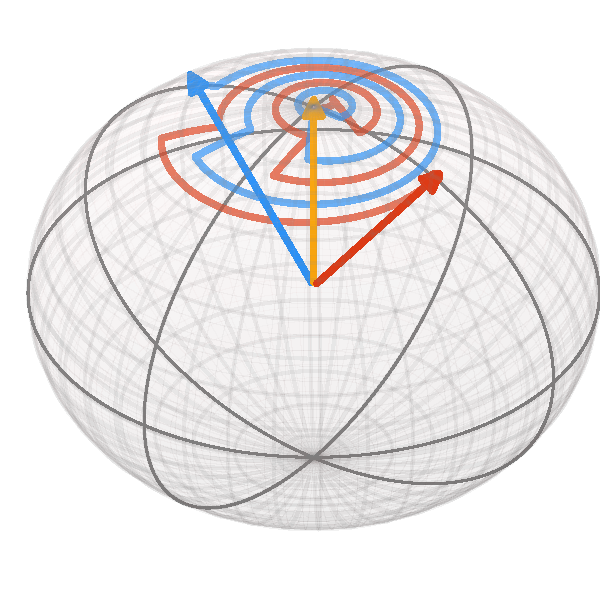
\includegraphics[width=\linewidth]{media/DDrf_2.pdf}
      \end{subfigure}
      \caption{Nuclear spin Bloch sphere trajectories conditioned on the electron state (blue: $m_s=0$, red: $m_s=-1$). (Left) Low $A_\perp$: the DDrf gate produces high-fidelity conditional rotation. (Right) High $A_\perp$: transverse hyperfine coupling distorts the trajectories, reducing gate fidelity.}
    \end{figure}

    The resulting two-qubit gate is a conditional rotation for each unit:
    where
    \begin{align}
      U_0 &= R_z (N(\omega_0 - \omega_1 )\tau) R_\varphi (N\Omega_{\text{rf}}\tau )\\
      U_1 &= R_z (N(\omega_0 - \omega_1 )\tau) R_\varphi (-N\Omega_{\text{rf}}\tau )
    \end{align}
    where $R_\varphi(\theta) = e^{-i\theta[\cos\varphi\, I_x + \sin\varphi\, I_y]}$.

  \end{block}

  \begin{block}{Hybrid DDrf Gate}
    \begin{figure}
      \centering
      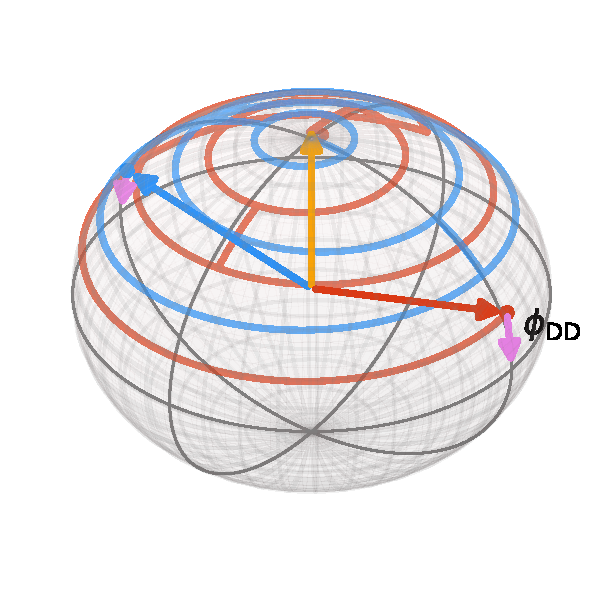
\includegraphics[width=0.35\linewidth]{media/DDrf_enhanced.pdf}
      \caption{Bloch sphere trajectories of the hybrid DDrf gate. The combined DD and rf contributions produce a larger conditional rotation angle $\phi_D$ (pink arrow), enabling faster operations than either mechanism alone.}
    \end{figure}

    The transverse hyperfine interaction ($A_\perp$) is exploited by the DD gate, and the rf driving ($\Omega$) by the DDrf gate. By allowing both contributions to act simultaneously, the hybrid approach can achieve:
    \begin{itemize}
      \item \textbf{Faster gate operations} through constructive combination of both driving mechanisms.
      \item \textbf{Broader applicability}, achieving high fidelity regardless of spin configuration.
    \end{itemize}

    To preserve the conditional operation arising from $A_\perp$ and the choice of $\tau$, we choose $\tau$ at the DD resonance condition $\vec\sigma_0 \cdot \vec{\sigma}_1 \simeq -1$, i.e.,
    $\tau = \frac{(2k + 1)\pi}{\omega_0 + \omega_1}, \quad k = 0, 1, 2, \ldots .$
    In the regime of small $A_\perp$, the two conditional rotation angles combine additively, resulting in conditional gate:
    \begin{align}
      U_0 &= R_x \!\left(N\bigl(\phi_\text{DD} + \Omega_{\text{rf}}\tau\bigr)\right)\\
      U_1 &= R_x \!\left(-N\bigl(\phi_\text{DD} + \Omega_{\text{rf}}\tau\bigr)\right)
    \end{align}
  \end{block}

  \begin{block}{References}

    \nocite{*}
    \footnotesize{\bibliographystyle{plainnat}\bibliography{poster}}

  \end{block}

\end{column}

\separatorcolumn
\end{columns}
\end{frame}

\end{document}
